\documentclass[a4paper]{jpconf}
\usepackage{graphicx}
\usepackage{url}
\usepackage{xspace}


\newcommand{\pd}{protoDUNE\xspace}
%\newcommand{\filesize}{5\,GB\ }

\begin{document}
\title{Design of the \pd experiment data management infrastructure}

\author{S Fuess$^1$, R Illingworth$^1$, M Mengel$^1$, A Norman$^1$, M Potekhin$^2$ and B Viren$^2$}

\address{$^1$ Fermi National Accelerator Laboratory, Batavia, IL 60510, USA}
\address{$^2$ Brookhaven National Laboratory, Upton, NY 11973, USA}

\ead{potekhin@bnl.gov}

\begin{abstract}
The Deep Underground Neutrino Experiment (DUNE) will employ a uniquely large 40kt Liquid Argon
Time Projection Chamber (LArTPC) as the main component of its Far Detector.
In order to validate this design and characterize the detector performance an
ambitious experimental program (called ``\pd'') has been
initiated which includes a beam test of large-scale prototypes of single-phase and dual-phase LArTPC
at CERN. The amount of data to be collected in this test is substantial and on par with the LHC experiments
in LHC Run 1. The protoDUNE experiment will require careful design of the DAQ, data handling and
data quality monitoring systems. There are also substantial requirements for data distribution
to a number of DUNE computing sites. We present our approach to solving these problems by
leveraging the design, expertise and components created for the LHC and Intensity Frontier
experiments. 
\end{abstract}

\section{Introduction}
The \pd program will help validate various DUNE technology aspects before proceeding with
the construction of the large-scale principal DUNE detectors at the Sanford Underground Research Facility \cite{cdrVol1, cdrVol4}.
The program is designed for measurements with a test beam provided by a dedicated target and beamline system
at the CERN SPS accelerator complex. It has the potential to be an important platform for realistic
Liquid Argon Time Projection Chamber (LArTPC) detector characterization (e.g. PID, shower response, etc.)
utilizing controlled conditions of a test-beam experimental setup. The program includes two
large LArTPC prototypes based on two different technologies --- single-phase and dual-phase TPCs.
The dual-phase prototype was given the official designation as a CERN experiment \textbf{NP02},
while the single-phase was designated as \textbf{NP04}. Both are to be deployed at CERN in 2017
and scheduled to take data in 2018.

While both apparatuses will share a few common computing infrastructure elements, their
respective design of DAQ and buffer as well as operations are largely independent.
The focus of this paper is on the data management for the
single-phase LArTPC (NP04)\,\cite{np04}. This detector  functions without amplification in the medium
(liquid Argon) and is in essence a very large ionization chamber equipped with a large
number of readout electrodes (wires), each with its own electronics chain.
In the DUNE design, the front-end electronics is situated within the cryostat and operates at cryogenic
temperatures in order to minimize noise (the so-called ``cold electronics design'').

Both NP02 and NP04 will be placed in an extension of the CERN North Area Experimental Hall.
There will be an enclosure with appropriately scaled power and cooling capacity to house the elements
of the \pd computing infastructure which need to be close to the detectors.
Each prototype will be have a dedicated optical fiber network connection to the CERN central storage facilities
located in the West Area campus of CERN. The nominal bandwidth of these dedicated network connections
will be 20\,Gbps for each experiment.


\section{LArTPC as a Data Source}

DUNE/\pd LArTPC design has the following characteristics which are common with
other recent detectors based on the same technology:
\begin{itemize}
\item High spatial granularity of readout (e.g. the electrode pattern), and the resulting high channel count
\item High digitization frequency (essential for precision)
\item Considerable duration of the readout window (a few ms), which is due to the relatively
low drift velocity of ionization electrons in Liquid Argon, of the order of mm/$\mu$s.
\end{itemize}

\noindent All these factors result in a considerable amount of data collected per single event readout.
A DUNE/\pd event may be compared to a stack of thousands of digital  snapshots of the signal
collected from the electrodes.  As detailed in Sec.\,\ref{sec:np04_data_rate} below,
instantaneous and average data rates in the data transmission chain are expected to be substantial, 
and the total amount of data to be produced by NP04 will be of the order of a few
petabytes (especially if one includes commissioning runs with cosmic rays).

A photon detector integrated into the TPC will also record data but its rate and volume are
expected to be quite small compared to the TPC data so it won't be addressed here.

There are data reduction (compression) techniques that are applicable to \pd raw data in order to reduce its size. 
Only the lossless algorithms will be applied during the compression of the NP04 raw data
(e.g. Huffman algorithm and others).

\section{The NP04 Data Characteristics}
\label{sec:np04_data_rate}
The following nominal parameters define the expected data rates and volume in NP04:
\begin{itemize}
\item TPC channel count: 15,360
\item Digitization frequency: 2MHz
\item Readout window: 5\,ms
\item Trigger rate: 100\,Hz
\item SPS spill time: 4.8\,s
\item SPS cycle: 16.8\,s
\item Compression: $\times$2
\end{itemize}
\noindent This results in the following nominal data characteristics:
\begin{itemize}
\item Instantaneous rate (in DAQ): 11.5\,GB/s
\item Average rate (including ingestion into mass storage): 3.3\,GB/s
\item Total data volume during the projected run period: 1.2\,PB (commisioning not included)
\item Buffer to store 3 days worth of data: 850\,TB

\end{itemize}


\section{Raw Data Flow in \pd}
\label{sec:raw_concept}
\subsection{DAQ and the Online Buffer}
Details of the DAQ design and Online Monitoring in \pd are outside of the scope
of this document but it is helpful to note a few details relevant for the topic at hand.

The DAQ has of a few interconnected layers of computers.
The ``outer layer'' of the system where the data is put together in a format
suitable for writing into files consists of about 10
 \textit{Event Builders} -- dedicated computers equipped with quad 10Gbps NICs to ensure the necessary
bandwidth. Interconnectivity is provided by a high-bandwidth switch such as Brocade ICX 7750
or equivanent. Their function is to assemble complete readout frames from data
fragments obtained from the inner layer of DAQ, the \textit{Board Readers}.

The Event Builders create the necessary file-level header information and write the
resulting data  to the \textit{Online Buffer} which is attached to the \pd DAQ. 
The design of this buffer is inspired by a system sucessfully employed in ATLAS experiment
and is based on a COTS storage hardware from DELL which features a high degree of redundnacy.
It is structured as 3 identical high-capacity storage system, i.e.~scales vertically. Each system contains
\begin{itemize}

\item Two front-end nodes (DELL R620 or similar)
\item Storage Controller (DELL MD3420 or similar)
\item Four expansion shelves (DELL MD1220 or similar)
\item A total of $\sim$120 HDDs
\end{itemize}

\noindent In addition to redundancy, the high HDD count is the main factor which allows
to sink \pd data to the disk at the high rate according to the experiment plan (Sec.\,\ref{sec:np04_data_rate})
and have enough headroom for robust operation.


A backup (auxiliary) option is to implement the buffer as a a XRootD \cite{xrootd} cluster
that may be deployed on existing general purpose hardware provided by the \textit{CERN
Neutrino Platform}\cite{cenf}.
A small prototype of such system has been tested.


\subsection{The logic of the Data Flow}
%%%%%%%%%%%%%%%%%%%%%%%%
\begin{figure}[tbh]
\centering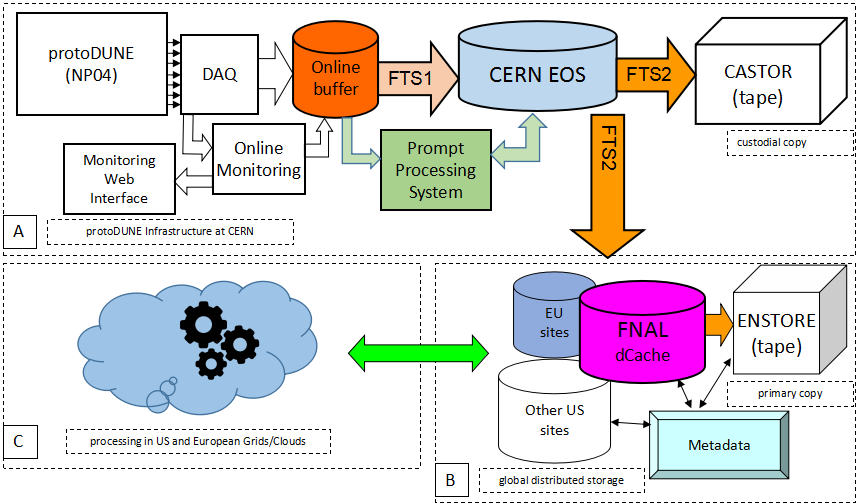
\includegraphics[width=0.85\linewidth]{figures/protoDUNE_data_flow_2017_v1.png}
\caption{\label{fig:raw_concept}Conceptual diagram of the flow of raw data in \pd}
\end{figure}
%%%%%%%%%%%%%%%%%%%%%%%%

In the following, we shall consider handling and management of the raw data after it is
written by the Event Builders to the Online Buffer.  Conceptual diagram of the raw data
flow in \pd is presented in Fig.\ref{fig:raw_concept} which shows the general logic of data flow
and also reflects the central role of the EOS system at CERN (the high-performance distributed
disk storage \cite{eos}) in the raw data management scheme.
Reliance on EOS is motivated by the experience and architecture of the LHC experiments
as well as the \pd data characteristics presented above in Sec.\,\ref{sec:np04_data_rate}.

The elements in this diagram which contain ``FTS'' in their label correspond to components and
instances of the \textit{Fermi File Transfer Service} -- FTS for short \cite{fts} -- which transports
data between a predefined endpoints.
There is more than once instance of FTS in the \pd data transmission chain. One instance (labeled ``FTS1''
in the diagram) is responsible for moving the data from the Online Buffer into EOS. The second instance
-- ``FTS2'' --  copies the data after is has arrived to EOS to tape storage at CERN (the CASTOR
system~\cite{castor}). It is also tasked with transmitting the data to Fermilab 
where it is placed
in a dCache~\cite{dcache} storage cluster. A secondary tape copy is then created at Fermilab
using the data resident in dCache as the source. Other participating data centers may also
receive their copies of raw data from this FTS instance.

In both cases an FTS agent is triggered by arrival of files to a designated
storage location which is expected to be accessible in a POSIX-like  mode.
It effectively servs as a ``dropbox'', i.e.\,files are picked up
for transfer asyncronously based on certain criteria (such as the filename pattern etc).
The Fermi FTS contains functionality which allows for completely automatic operation
including error handling, transmission retries, monitoring etc.

An important part of the FTS functionality is its interface to and integration with 
the \textit{SAM} Metadata system deployed at FNAL which serves the needs of a few
experiments in both HEP and Intensity Frontier domains. In addition to essential file catalog
functionality, SAM has extensive storage management
capabilities covering both disk (e.g.\,dCache) and tape (e.g.\,FNAL Enstore) types of storage.
% Working in tandem, FTS and SAM allow
The most common way
to associate metadata with a file in SAM is to package it as an auxiliary file in JSON format,
following certain naming convention. This file is then automatically detected by FTS
and records in SAM are created in accordance with its content.

\subsection{Transfer Protocols}
A number of protocols are supported by both EOS and FTS inclusing XRootD, gridFTP
and third-party transfers. Prime candidate for \pd is XRootD which has proven scalability
and reliability.

In addition to serving as the principal staging area from which the data is copied to
tape storage at CERN and from which it is transmitted to FNAL, 
EOS will also be used to provide trasparent access to data to the prompt processing system
in order support the Data Quality Moniotring (DQM) in \pd as explained in Sec.\,\ref{sec:dqm}.
Its XRootD interface makes it a particularly attractive option.

\section{Data Quality Monitoring}
\label{sec:dqm}
Data Quality Monitoring (DQM) plays an imporant role in \pd.
Its goal is to generate time-critical information on a short time
scale needed to ascertain the condition
and performance of both the detector and the DAQ,
in order for operators to quickly detect problems, take action and prevent loss
of useable data and/or beam time.

DQM consists of two parts,  the low latency Online Monitoring (OM)
system which is engineered as a component of DAQ, and
the ``prompt processing system''. This is reflected in the diagram
in Fig.\ref{fig:raw_concept}.
These systems are complementary to each other but operate
in different enviroment and on a different time scale.
The benchmark turnaround time for ``prompt processing'' jobs 
is set roughly at 10\,min, with actual numbers depending on
finalized content of the payload, while Online Monitoring aims
to provide response on the scale of seconds an in general under a minute.

The prompt processing system processes only a small fraction of the data
but can potentially perform more sophisticated calculations since it is
easier to scale out its CPU capabilities.



\section*{References}
\begin{thebibliography}{9}

\bibitem{cdrVol1} DUNE CDR Vol 1 -- The LBNF and DUNE Projects\\
\url{http://arxiv.org/abs/1601.05471}

\bibitem{cdrVol4} DUNE CDR Vol 4 -- The DUNE Detectors at LBNF\\
\url{http://arxiv.org/abs/1601.02984}

\bibitem{np04} 
Yearly report on ProtoDUNE Single Phase NP04 (2016)\\
\url{https://cds.cern.ch/record/2144868}

\bibitem{xrootd}
{XRootD}\\
\url{http://www.xrootd.org}

\bibitem{cenf}
{CERN Neutrino Platform}\\
\url{http://home.cern/about/experiments/cern-neutrino-platform}



\bibitem{eos}
{The CERN Exabyte Scale Storage}\\
\url{http://information-technology.web.cern.ch/services/eos-service}

\bibitem{fts}
{The Fermilab File Transfer System}\\
\url{http://cd-docdb.fnal.gov/cgi-bin/RetrieveFile?docid=5412&filename=datamanagement-changeprocedures.pdf&version=1}

\bibitem{castor}
{CASTOR -- CERN Advanced STORage manager}\\
\url{http://castor.web.cern.ch/}

\bibitem{dcache}
{dCache.org}\\
\url{https://www.dcache.org/}

\bibitem{sam}
{A data handling system for modern and future Fermilab experiments}\\
\url{http://iopscience.iop.org/1742-6596/513/3/032045}

\end{thebibliography}





\end{document}


